\FloatBarrier
\subsection{Breakup Auroral Arcs}\label{sec:breakup}
Highly dynamic events may combine several auroral morphologies, driven by diverse acceleration mechanisms, yielding multiple plasma turbulence types in close spatiotemporal proximity.
These events are difficult to interpret with instruments smearing in time by a factor of 100..1000 times greater than the ground-observable timescales.
It is also impractical to have a human manually initiating recording during extended observations.
This fact motivates the automatic Alfvénic aurora discrimination algorithms cited in section~\ref{sec:hist}.

A canonical example of such an event motivating the HiST system was the auroral breakup of March 23, 2007 shown in Figure~\ref{fig:20070323}.
\begin{figure}
    \noindent\includegraphics[width=0.9\columnwidth,trim=0 383 0 10,clip]{gfx/2007-03-23/2007-03-23}
    \vspace{0.1cm}
    
    % psd ion-line
    \includegraphics[width=0.3\columnwidth,trim=0 55 0 0]{gfx/2007-03-23/acfslice_alternatingcode2007-03-2311-20-08}
    \includegraphics[width=0.3\columnwidth,trim=0 55 0 0]{gfx/2007-03-23/acfslice_alternatingcode2007-03-2311-20-23}
    \includegraphics[width=0.3\columnwidth,trim=0 55 0 0]{gfx/2007-03-23/acfslice_alternatingcode2007-03-2311-20-39}
    
    \vspace{-0.5cm}
    \hspace{0.1cm}(f)\hspace{0.275\columnwidth}(g)\hspace{0.275\columnwidth}(h)
    \vspace{0.1cm}
    
    % psd plasma-line
    \includegraphics[width=0.45\columnwidth,trim=0 60 0 0]{gfx/2007-03-23/plasmaDOWNslice2007-03-2311-20-08}
    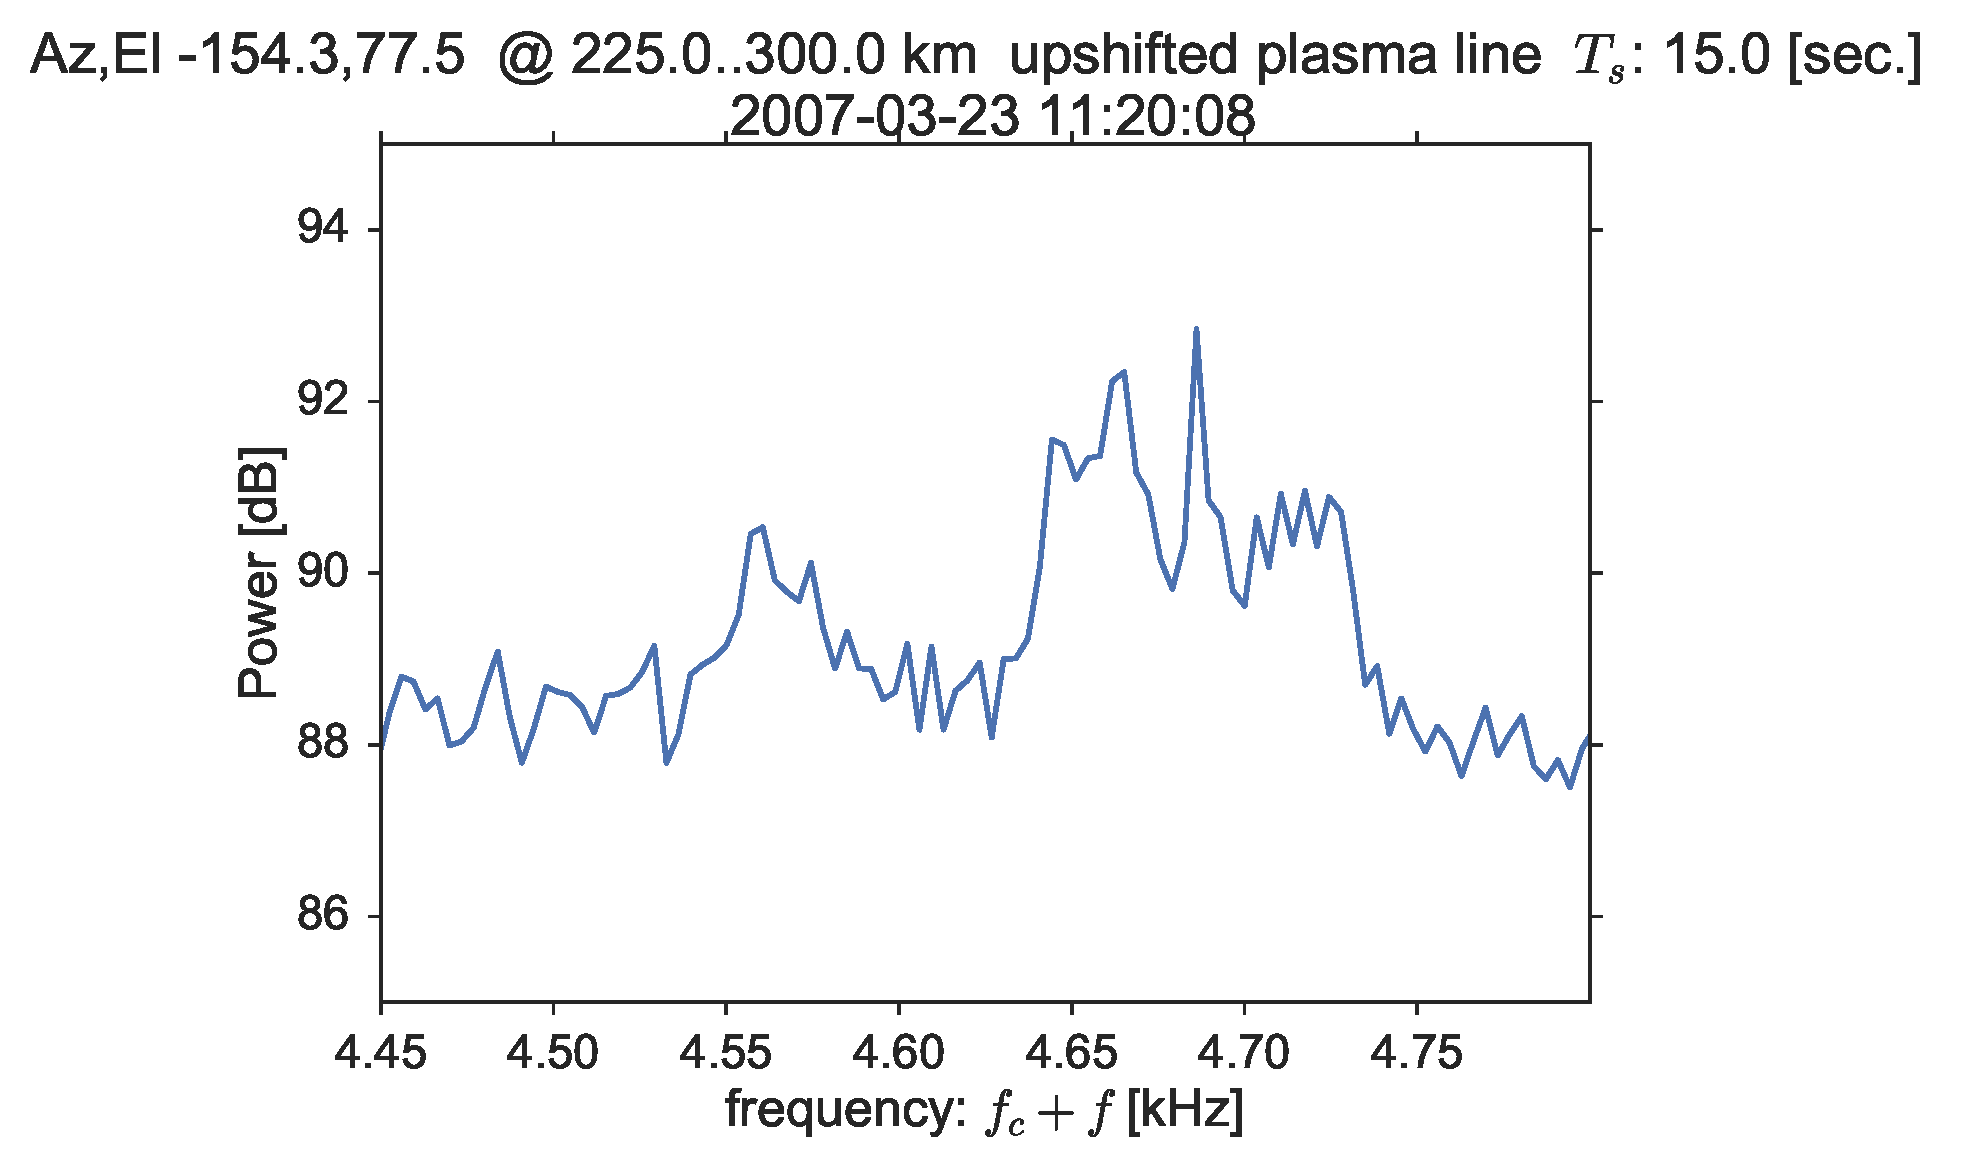
\includegraphics[width=0.45\columnwidth,trim=0 60 0 0]{gfx/2007-03-23/plasmaUPslice2007-03-2311-20-08}
    
    \vspace{-0.5cm}
    \hspace{0.5cm}(i)\hspace{0.425\columnwidth}(j)
    \vspace{0.5cm}
    
    \caption{Substorm breakup: highly dynamic aurora on 23 March 2007. 
        Low-altitude NEIALs observed corresponding to (a,c,f,i,j) with possible Farley-Buneman instability in the E-region. 
        Streaming upflow corresponding to (d,h).
    Strong Langmuir turbulence corresponding to (c,f,g). }\label{fig:20070323}
\end{figure}
The PF-DMSP spectra ratio $I_{6300}/I_{4278}$ in Figure~\ref{fig:mspratio0323} dips as low as 0.02 during the breakup, indicating a large flux with $E_0 > \unit[10]{keV}$ according to \citet{rees1974}.
\begin{sidewaysfigure}\centering
    \includegraphics[width=0.85\linewidth]{gfx/2007-03-23/msp-ratio}
    \caption{PF-DMSP spectral ratio breakup event 2007 March 23 11:22 UTC.
        The ratio $I_{6300}/I_{4278}$ dips as low as 0.02 during the breakup, indicating a large flux with $E_0 > \unit[10]{keV}$ according to \citet{rees1974}.}
    \label{fig:mspratio0323}
\end{sidewaysfigure}
The $I_{5577}/I_{4278}$ in Figure~\ref{fig:mspratio0323-5577} dips as low as 1 during the breakup, also indicating a large flux with $E_0 > \unit[10]{keV}$ according to \citet{rees1974}.
\begin{sidewaysfigure}\centering
    \includegraphics[width=0.85\linewidth]{gfx/2007-03-23/msp-ratio-5577}
    \caption{PF-DMSP spectral ratio breakup event 2007 March 23 11:22 UTC.
        The ratio $I_{5577}/I_{4278}$ dips as low as 1 during the breakup, indicating a large flux with $E_0 > \unit[10]{keV}$ according to \citet{rees1974}.}
    \label{fig:mspratio0323-5577}
\end{sidewaysfigure}
The GIMA magnetometers data surrounding this event is shown in Figure~\ref{fig:20070323mag}, with the expected strong perturbation near the event time.
\begin{figure}
    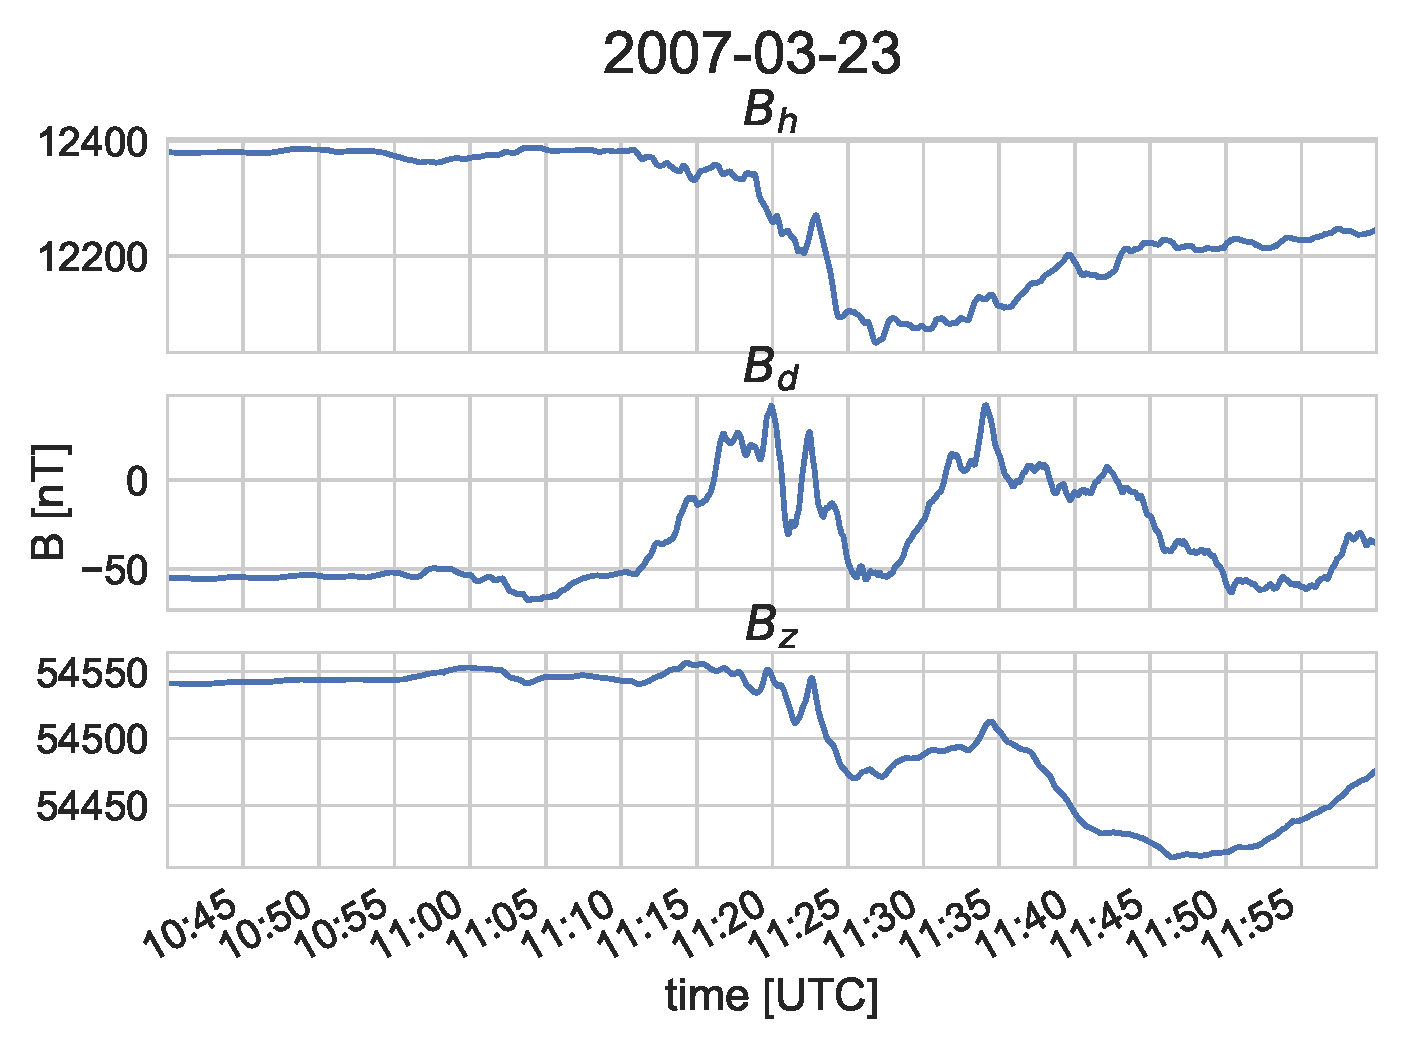
\includegraphics[width=\columnwidth]{gfx/2007-03-23/mag}
    \caption{Strong B-field perturbance due to substorm on 2007-03-23 near 11:20 UTC.}
    \label{fig:20070323mag}
\end{figure}

This was an exceptionally intense breakup event.
This magnificent substorm breakup had splitting arcs embedded in the wildly dynamic behavior captured by PFISR and a single BG3-filtered EMCCD camera. 
This event has been analyzed in detail by \citet{semeter2008,akbari2012}.
